\documentclass[border=10pt]{standalone}

\usepackage{tikz}
\usepackage{tikzsymbols}
\usetikzlibrary{calc,patterns,shapes.geometric}

\def\centerarc[#1](#2)(#3:#4:#5){\draw[#1] ($(#2)+({#5*cos(#3)},{#5*sin(#3)})$) arc (#3:#4:#5);}

\begin{document}
	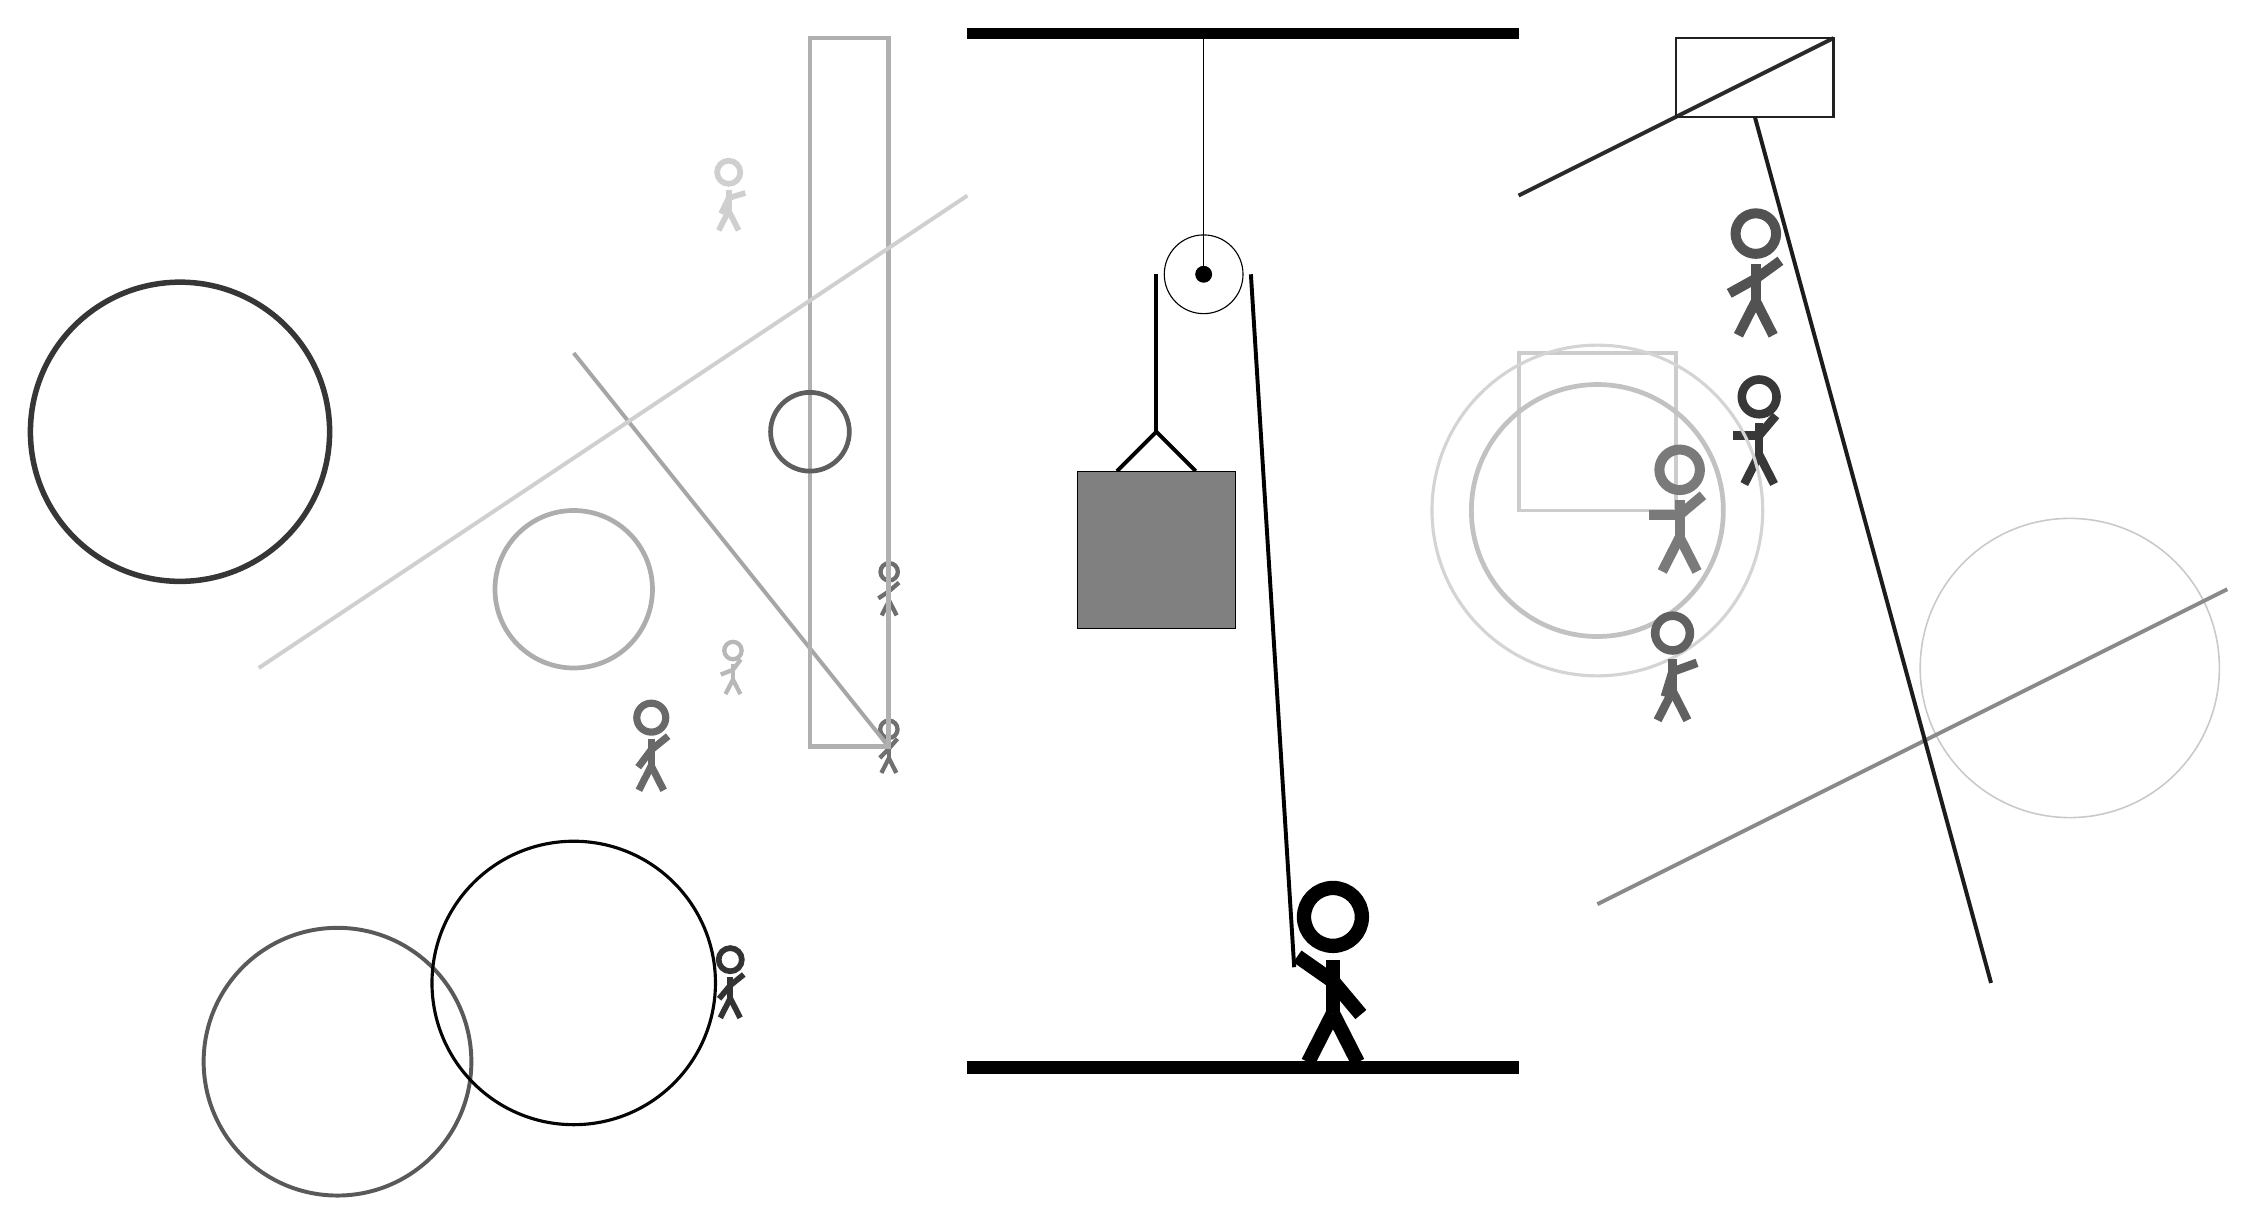
\begin{tikzpicture}
		%%%%% START %%%%%
		
		\draw[fill=black] (-2, 10) rectangle (5, 10.125);
		
		\draw (1, 7) circle (0.5);
		\draw[fill=black] (1, 7) circle (0.1);
		\draw (1, 10) -- (1, 7);
		
		\draw[line width=0.5mm] (-0.1, 4.5) -- (0.4, 5.0) -- (0.9, 4.5);
		\draw[fill=black!50] (-0.6, 4.5) rectangle (1.4, 2.5);
		
		\draw[line width=0.5mm] (0.4, 7) -- (0.4, 5.0);
		\centerarc[line width=0.5mm](1, 7)(0:180:0.6);
		\draw[line width=0.5mm](1.6, 7) -- (2.15, -1.8);
		
		\node at (2.6, -1.9) {\Strichmaxerl[10][-35][-50]};
		
		\node[line width=0.5mm, color=black!56] at (-3, 1) {\Strichmaxerl[3][46][49]};
		
		\node[line width=0.6mm, color=black!57] at (-3, 3) {\Strichmaxerl[3][34][41]};
		\draw[line width=0.5mm, color=black!20] (5, 6) rectangle (7, 4);
		\draw [line width=0.2mm, color=black!21](12, 2) circle (1.9);
		
		\node[line width=0.2mm, color=black!52] at (7, 4) {\Strichmaxerl[7][0][40]};
		\draw[line width=0.5mm, color=black!84](9, 10) -- (5, 8);
		\node[line width=0.2mm, color=black!68] at (8, 7) {\Strichmaxerl[7][29][36]};
		\draw[line width=0.5mm, color=black!35](-7, 6) -- (-3, 1);
		\draw [line width=0.6mm, color=black!24](6, 4) circle (1.6);
		\draw[line width=0.6mm, color=black!31] (-3, 10) rectangle (-4, 1);
		\node[line width=0.6mm, color=black!19] at (-5, 8) {\Strichmaxerl[4][64][17]};
		
		\draw [line width=0.7mm, color=black!79](-12, 5) circle (1.9);
		\draw [line width=0.6mm, color=black!32](-7, 3) circle (1.0);
		\node[line width=0.3mm, color=black!78] at (8, 5) {\Strichmaxerl[6][0][50]};
		\node[line width=0.3mm, color=black!59] at (-6, 1) {\Strichmaxerl[5][53][39]};
		\draw[line width=0.5mm, color=black!19](-2, 8) -- (-11, 2);
		
		\draw[line width=0.3mm, color=black!87] (7, 10) rectangle (9, 9);
		\node[line width=0.7mm, color=black!28] at (-5, 2) {\Strichmaxerl[3][21][53]};
		\draw [line width=0.6mm, color=black!63](-4, 5) circle (0.5);
		\draw [line width=0.5mm, color=black!65](-10, -3) circle (1.7);
		\draw [line width=0.4mm, color=black!98](-7, -2) circle (1.8);
		
		\draw [line width=0.4mm, color=black!17](6, 4) circle (2.1);
		\node[line width=0.4mm, color=black!80] at (-5, -2) {\Strichmaxerl[4][50][39]};
		\draw[line width=0.5mm, color=black!46](6, -1) -- (14, 3);
		\draw[line width=0.5mm, color=black!89](8, 9) -- (11, -2);
		\node[line width=0.2mm, color=black!62] at (7, 2) {\Strichmaxerl[6][73][20]};
		
		\draw[fill=black] (-2, -3) rectangle (5, -3.15);
		
		%%%%% END %%%%%
	\end{tikzpicture}
\end{document}